\section{Doelstelling}

Op het moment zit er een Beckhoff \gls{AX5140} servo drive in de testkast gebouwd
voor het aansturen van de motoren. De parameters die in deze drive zitten kunnen
momenteel alleen de servomotor HQL100X aansturen. Andere motoren kunnen
niet worden aangestuurd met deze parameters omdat deze motoren bijvoorbeeld
een andere encoder hebben, andere /gls{PID}-instellingen of de motor werkt simpelweg
volgens een ander principe (asynchrone of synchrone servo). De \gls{AX5140} heeft
meer dan 400 parameters de meeste hiervan kunnen worden aangepast. Naast deze
parameters zijn er ook nog parameters instelbaar aan de \gls{PLC} kant in de zogehete
\gls{NC}-task die verantwoordelijk is voor het aansturen van de drive.

\vspace{0.5cm}

Ook is het testprotocol van Voortman op de spindels niet erg geavanceerd zo
worden motoren alleen aangestuurd naar een bepaald tourental voor een bepaald
aantal seconden waarbij er gelet wordt of de motor niet te veel trilt en of deze niet
te warm wordt. Zij kwantificeren deze waardes niet het is daarom erg lastig om
aantoonbaar de motor te beoordelen op zijn prestaties.

\vspace{0.5cm}

De wens is daarom vanuit Voortman om uit te zoeken welke parameters relevant
zijn voor wanneer er een motor gewisseld wordt en welke waardes dit moeten zijn
voor de motoren die zij willen gaan testen. Met daarbij een programma die ervoor
kan zorgen dat deze parameters eenvoudig naar de drive kunnen worden geschreven.
Daarnaast zou het mooi zijn als er uitgezochtwordtwatVoortman wil gaan testen aan
de motoren en wat hiervoor eventueel voor nodig is zoals een trilling sensor die de
trillingen van de spindel kan meten zodat de testen op de motoren gekwantificeerd en
gedocumenteerd kunnen worden in plaats van de huidige manier van testen waarbij
er niks aan de motor gemeten wordt.

\begin{figure}[H]
	\centering
	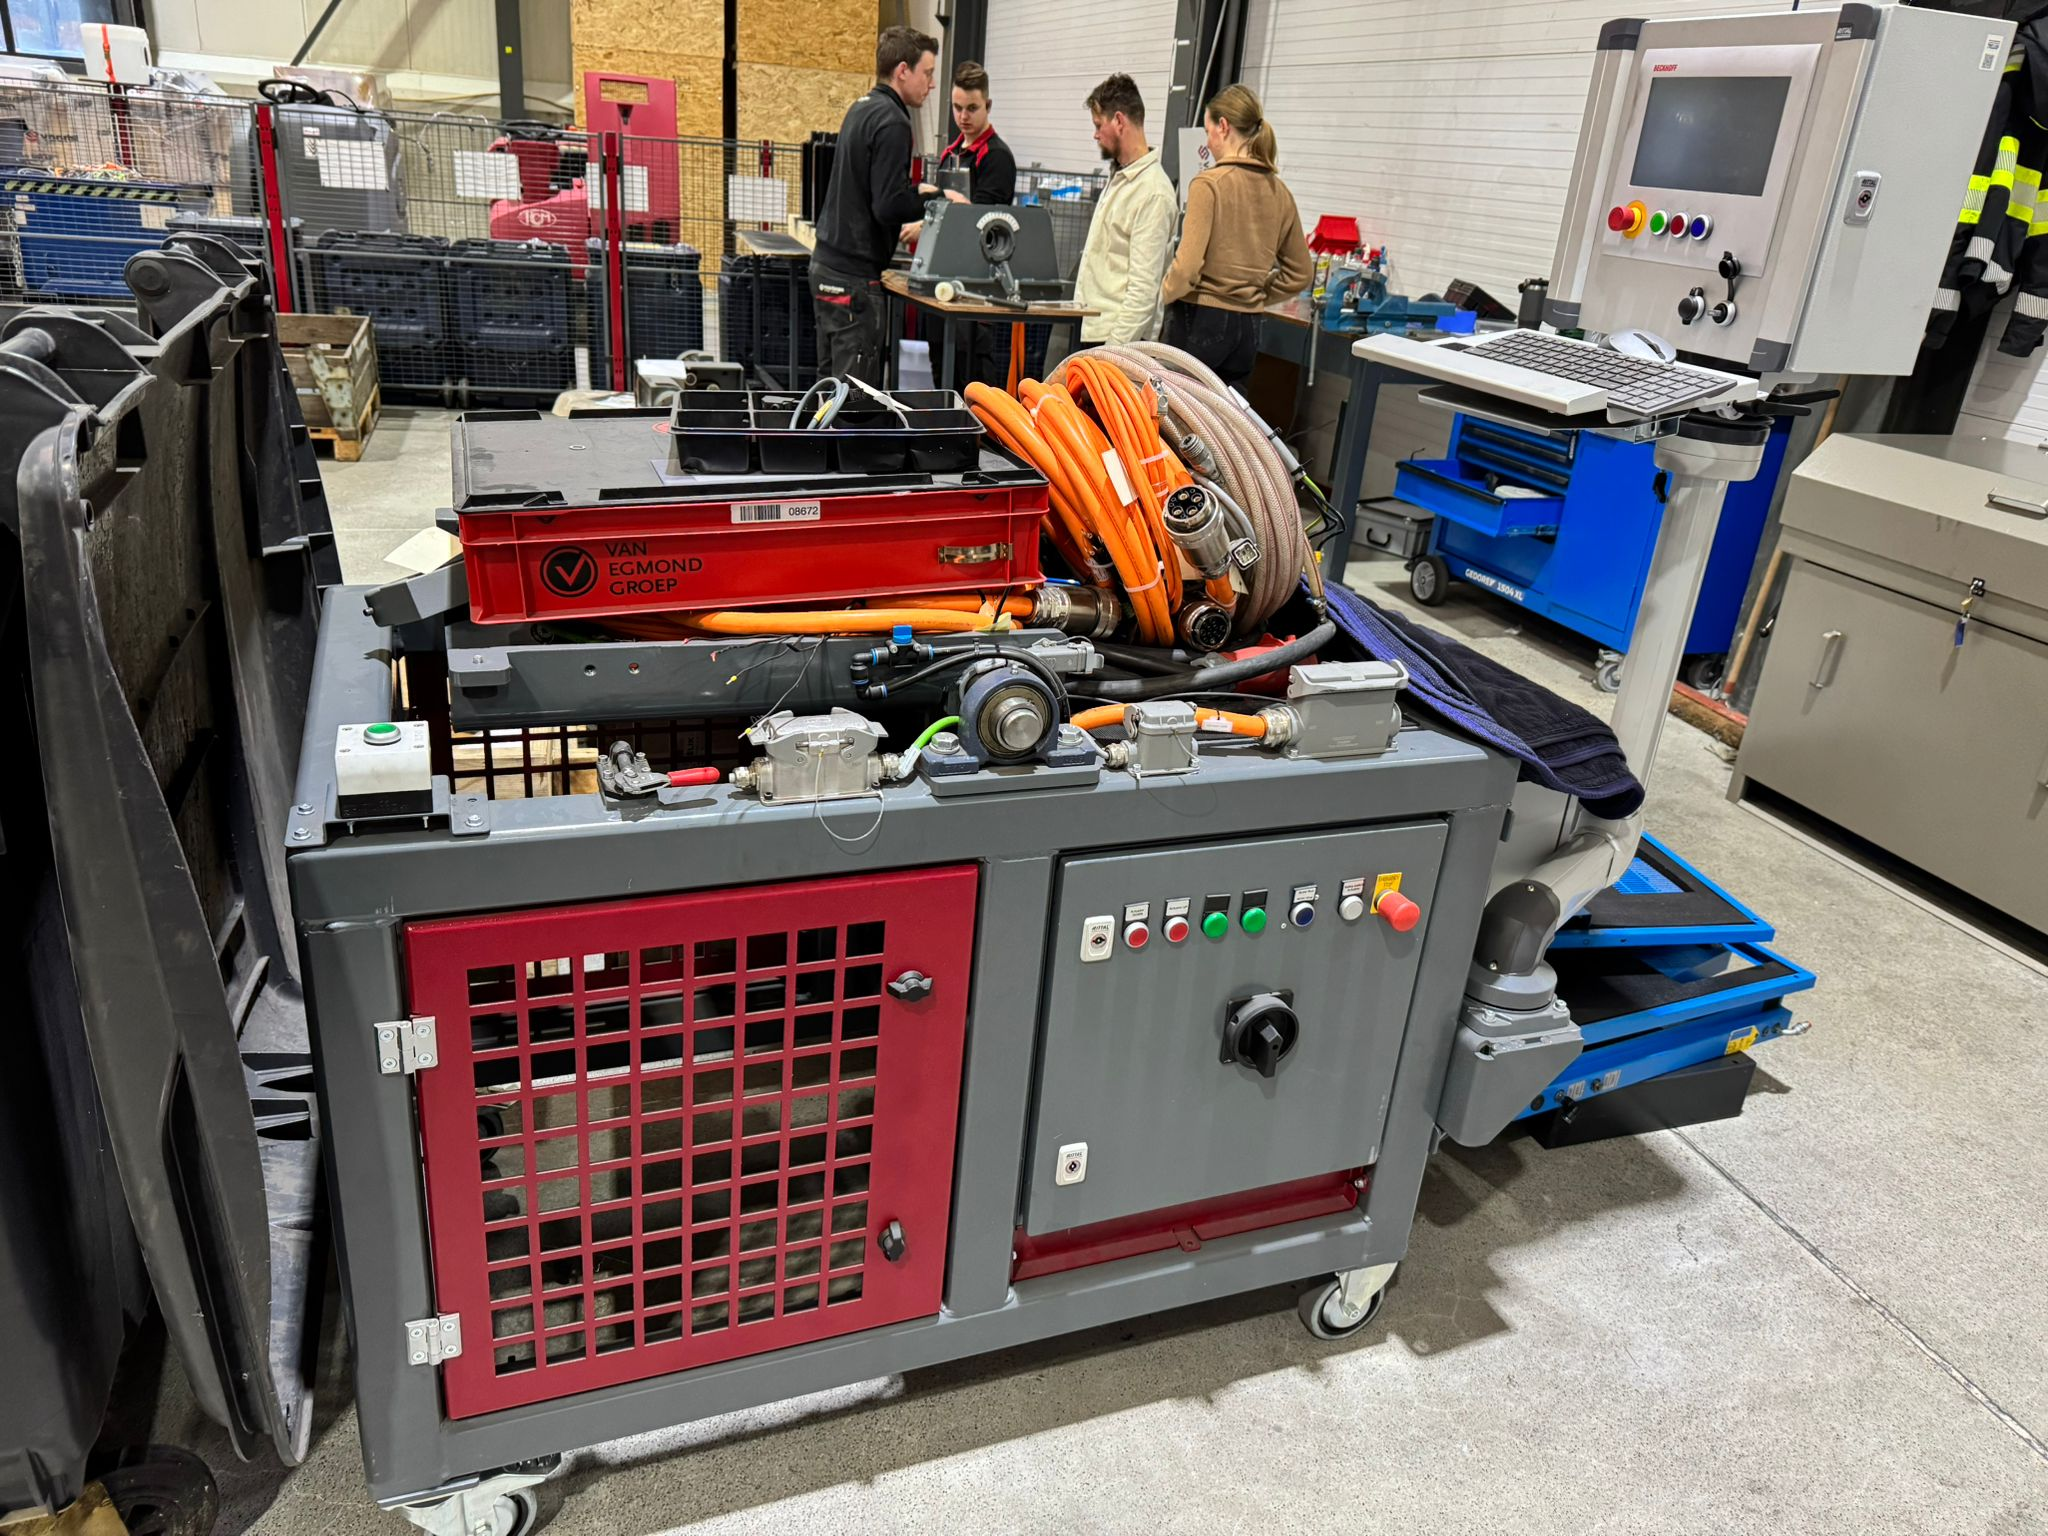
\includegraphics[width=0.7\linewidth]{TestKast}
	\label{fig:Testkast}
	\caption{De testkast in kwestie}
\end{figure}